\section*{Separación de datos}
Antes de comenzar a entrenar el modelo, es indispensable separar los datos en conjuntos de entrenamiento y evaluación.
Al finalizar el entrenamiento, estimaremos la performance de nuestro modelo con los datos de evaluación, para lograr estimar un resultado  lo mas cercano a la realidad posible.

Nuestra decisión fue separar un 15\% de los datos para evaluación y el sobrante 85\% para entrenamiento.
Como queremos que nuestro modelo sea entrenado y validado con las mismas frecuencias en clases,
nos encargamos de que la separación mantenga la misma proporción de clases, además de realizar un \textit{shuffle} de los datos previo a la separación.


\begin{figure}[H]
    \centering
    \subfloat[\centering Dataset completo \label{fig:classDistrCompl}]{
        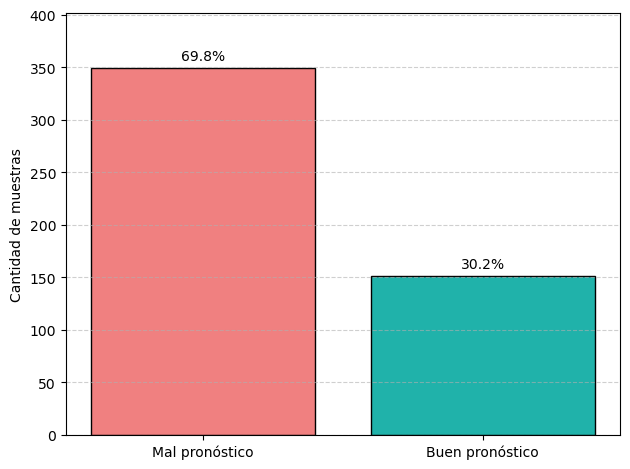
\includegraphics[width=0.25\linewidth]{img/class_distr_compl.png}
    }
    \hspace{0.05\linewidth}
    \subfloat[\centering Datos de entrenamiento \label{fig:distr1}]{
        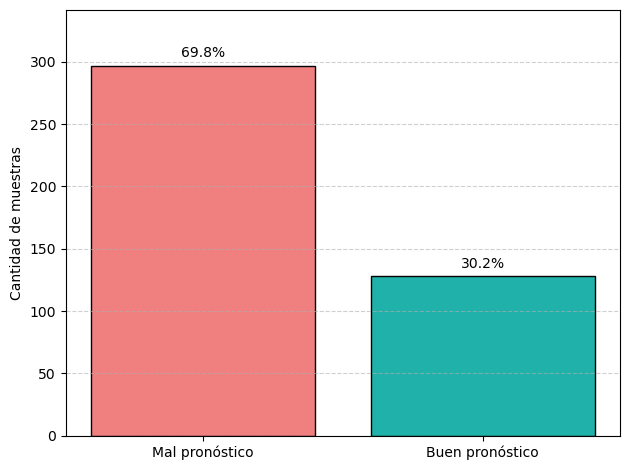
\includegraphics[width=0.25\linewidth]{img/class_distr_train.png}
    }
    \hspace{0.05\linewidth}
    \subfloat[\centering Datos de evaluación \label{fig:distr2}]{
        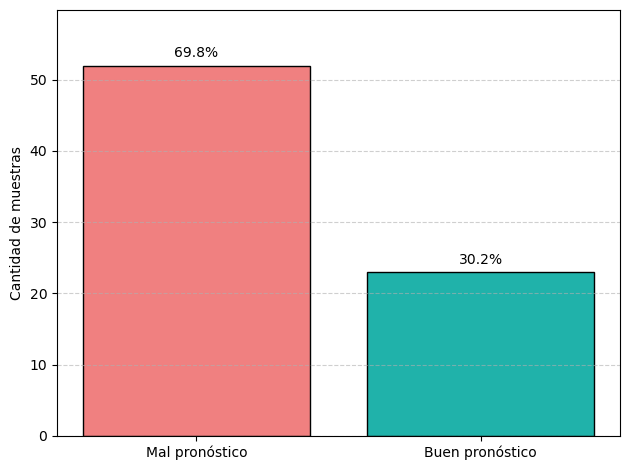
\includegraphics[width=0.25\linewidth]{img/class_distr_eval.png}
    }
    \caption{Distribución de clases en los distintos conjuntos de datos}
    \label{fig:distr}
\end{figure}


En \ref{fig:classDistrCompl} podemos ver como el dataset completo tiene un 69,8\% de datos etiquetados por mal pronostico y un 30,2\% de buen pronostico, y en \ref{fig:distr1} y \ref{fig:distr2} vemos como el conjunto de entrenamiento y evaluación 
mantienen la misma proporción de clases que el dataset completo.
